\documentclass[11pt]{article}
\usepackage[margin=1in]{geometry}
\usepackage{amsmath,amssymb,amsthm,mathtools}
\usepackage{booktabs}
\usepackage{graphicx}
\usepackage{tikz}
\usetikzlibrary{arrows.meta,positioning,backgrounds}
\usepackage{hyperref}
\usepackage{longtable}
\usepackage{array}
\newtheorem{theorem}{Theorem}
\newtheorem{lemma}[theorem]{Lemma}
\newtheorem{proposition}[theorem]{Proposition}
\newtheorem{corollary}[theorem]{Corollary}
\newtheorem{definition}[theorem]{Definition}
\newtheorem{remark}[theorem]{Remark}
\newenvironment{sourceresult}[1]{\par\medskip\noindent\textbf{#1.}\ \itshape}{\par\medskip}
\sloppy
\emergencystretch=3em

\title{Formal Verification Report: Theorem 1.1\\[0.5em]{\large Source: Eliahou, S. (1993). The 3x+1 problem: new lower bounds on nontrivial cycle lengths. Discrete Mathematics 118(1-3), 45-56.}}
\author{Black Swan Labs FCVE \\ ledger through EVENT-017}
\date{2026-09-19}
\begin{document}
\maketitle

\noindent\textbf{Trust Statement.} The formal result was checked using Lean 4.28.0 under the pinned project environment (Mathlib v4.28.0 pin). The theorem CLAIM-001 was kernel-checked with axiom footprint Classical.choice, Quot.sound, propext. Independent checking status is INDEPENDENTLY\_CHECKED. Computational/adversarial testing produced: COMPUTATIONALLY\_SUPPORTED (diagnostic only). The remaining trust limitations are: The proof uses Classical.choice; it is a classical proof; The repository, commit and toolchain were captured after the run (on 2026-09-19), not recorded during it; they describe the project as it is now, and the commit matches the one named in the run's own notes; The recorded result of EVENT-006 refers to a log or receipt that is not part of this report (``see prior receipt for full log''), so that material cannot be inspected here; No counterexample was sought against the underlying nontrivial-cycle claim; that is infeasible; The independent check used patched copies of lean4export and nanoda (huge-literal handling). This report does not claim that computational testing constitutes formal proof or that formalization alone establishes the truth of the original informal statement.

\begin{abstract}
This report documents the formal verification of Theorem 1.1 (CLAIM-001) under the Formal Claim Verification Engine. Recorded: build PASS (8033/8033 jobs; see prior receipt for full log); axiom footprint Classical.choice, Quot.sound, propext  [reported: Classical.choice]; independent check INDEPENDENTLY\_CHECKED. Computational testing is diagnostic and is not proof. Section 17 states the status the recorded evidence permits; the governance decision is recorded separately, after this report.
\end{abstract}

\section{Mathematical Statement}
\begin{sourceresult}{Theorem 1.1}
Let \ensuremath{\Omega} be a nontrivial cycle of T. Provided min \ensuremath{\Omega} > 2\textasciicircum{}40, we have Card \ensuremath{\Omega} = 301994a + 17087915b + 85137581c, where a,b,c are nonnegative integers, b>0, and ac=0. In particular, the smallest admissible values for Card \ensuremath{\Omega} are 17087915, 17389909, 17691903, and so on.
\end{sourceresult}
Source: Eliahou, S. (1993). The 3x+1 problem: new lower bounds on nontrivial cycle lengths. Discrete Mathematics 118(1-3), 45-56.. Source location: eliahou-collatz.pdf, pages 46, 55-56.

\noindent Facts the statement relies on:
\begin{itemize}
\item p\_13 = 301994, q\_13 = 190537 (Table 1, n=13)
\item p\_15 = 17087915, q\_15 = 10781274 (Table 1, n=15)
\item p\_16 = 85137581, q\_16 = 53715833 (Table 1, n=16)
\item K(2\textasciicircum{}39) = p\_13 = 301994 (p.55: the transition point tr(13,0) is near 2\textasciicircum{}39)
\item K(2\textasciicircum{}40) = K(2\textasciicircum{}48) = p\_15 = 17087915 (p.55: the next transition point tr(15,0) is near 2\textasciicircum{}48)
\item p\_16/q\_16 < log2(3) < p\_15/q\_15 < log2(3+2\textasciicircum{}-40) < p\_13/q\_13 (p.55, from Tables 1-2)
\end{itemize}
\section{Definitions and Assumptions}
\subsection*{Definitions}
\begin{itemize}
\item T: N -> N, T(n) = n/2 if n even, (3n+1)/2 if n odd (p.45)
\item trajectory: Omega(n) = \{n, T(n), T\textasciicircum{}(2)(n), ...\} (p.45)
\item cycle of length k: a trajectory Omega with T\textasciicircum{}(k)(x)=x for all x in Omega, where k = Card Omega (p.45) -- 'length k' is DEFINED to equal Card Omega, not merely correlated with it
\item trivial cycle: Omega(1) = \{1,2\}, the only cycle containing 1 under the 3x+1 conjecture (p.45)
\item theta = log2(3), an irrational number; [a0,a1,a2,...] its continued fraction expansion (p.50)
\item p\_n/q\_n: the principal convergents to theta, defined recursively by p\_n=a\_n*p\_\{n-1\}+p\_\{n-2\}, q\_n=a\_n*q\_\{n-1\}+q\_\{n-2\} (p.51, eq 3.2)
\item Farey pair: (p/q),(p'/q') with pq'-p'q=+-1 (p.49)
\item K(m): the smallest positive integer k such that log2(3) < k/l <= log2(3+1/m) for some positive integer l (p.48, p.52)
\end{itemize}
\subsection*{Source assumptions}
\begin{itemize}
\item \textbf{SA-001} \ensuremath{\Omega} is a nontrivial cycle of T (i.e. \ensuremath{\Omega} is not the trivial cycle \{1,2\})
\item \textbf{SA-002} min \ensuremath{\Omega} > 2\textasciicircum{}40
\item \textbf{SA-003} theta = log2(3) is irrational
\item \textbf{SA-004} Standard theory of continued fractions and Farey pairs (attributed to Wallis 1685, via reference [1])
\end{itemize}
\subsection*{Formalization assumptions}
\begin{itemize}
\item \textbf{FA-001} A 'cycle of length L' is represented in Lean as a structure CollatzCycle L with an index type Fin L -> N and a cyclic step relation, which does NOT by itself guarantee the L indices map to L distinct integers.
\item \textbf{FA-002} Real-number computations (log2, division) are represented via Mathlib's Real.logb and instances of classical real-number axioms (propext, Classical.choice, Quot.sound).
\end{itemize}
\subsection*{Computational assumptions}
\begin{itemize}
\item \textbf{CA-001} Table 1 and Table 2's specific large-integer values (p\_13=301994, p\_15=17087915, p\_16=85137581, and the continued-fraction coefficients a\_n) were computed by the paper's author on a 1993-era Toshiba 1600 using muLISP, per the Acknowledgements (p.56). This is a computation performed OUTSIDE Lean, by the original 1993 paper.
\end{itemize}
\section{Proof Outline}
\begin{enumerate}
\item \textbf{step 1.} Corollary 2.3 (via Theorem 2.1 + definition of K,L): Card Omega >= K(min Omega), Card Omega1 >= L(min Omega)
\item \textbf{step 2.} Set k = Card Omega, l = Card Omega1. By Theorem 2.1, log2(3+M\textasciicircum{}-1) < k/l <= log2(3+m\textasciicircum{}-1); since M >= m > 2\textasciicircum{}40, k/l lies in the open interval (log2(3), log2(3+2\textasciicircum{}-40))
\item \textbf{step 3.} That interval sits strictly between three specific convergents: p\_16/q\_16 < log2(3) < p\_15/q\_15 < log2(3+2\textasciicircum{}-40) < p\_13/q\_13
\item \textbf{step 4 case split.} k/l falls into exactly one of three regions, each handled by Lemma 3.1 (Farey-pair intermediate-fraction structure): (i) k/l in (p\_16/q\_16, p\_15/q\_15) => k = p\_15*b + p\_16*c for some b,c in N; (ii) k/l = p\_15/q\_15 exactly => k = p\_15*b for some b in N; (iii) k/l in (p\_15/q\_15, p\_13/q\_13) => k = p\_13*a + p\_15*b for some a,b in N
\item \textbf{step 5.} Since the three cases are mutually exclusive and each includes a nonzero p\_15 (=17087915) term, combining them gives Card Omega = 301994a + 17087915b + 85137581c with b>0 always, and a*c=0 because no single case ever produces both a nonzero a AND a nonzero c simultaneously
\end{enumerate}
\begin{sourceresult}{Lemma 2.2}
Let Omega, Omega1 be as above, and let k = Card Omega. Then prod\_\{n in Omega1\} (3+n\textasciicircum{}-1) = 2\textasciicircum{}k.
\end{sourceresult}
\begin{sourceresult}{Theorem 2.1}
Let Omega be a cycle of T, and let Omega1 subset Omega denote the subset of its odd elements. Then log2(3+M\textasciicircum{}-1) < Card(Omega)/Card(Omega1) <= log2(3+m\textasciicircum{}-1), where M=max Omega, m=min Omega. In fact, a sharper right inequality holds: Card(Omega)/Card(Omega1) <= log2(3+mu), where mu = (1/Card Omega1) * sum\_\{n in Omega1\} n\textasciicircum{}-1.
\end{sourceresult}
\begin{sourceresult}{Lemma 3.1}
Let p/q < p'/q' be a Farey pair. Then any intermediate fraction p/q < x/y < p'/q' with y>0 is of the form x/y = (ap+bp')/(aq+bq') where a,b are positive integers. In particular, x >= p+p' and y >= q+q'.
\end{sourceresult}
\begin{sourceresult}{Corollary 2.3}
Let Omega be a cycle of T, and let Omega1 subset Omega denote the subset of its odd elements. Then Card Omega >= K(min Omega), Card Omega1 >= L(min Omega).
\end{sourceresult}
\begin{sourceresult}{Theorem 3.2}
Let theta > 0 be irrational, theta' any number with theta < theta' < [theta]+1. If k,l are positive integers with theta < k/l <= theta', and either k or l is minimal for this property, then k/l is one of the upper convergents to theta -- precisely, the largest upper convergent <= theta'.
\end{sourceresult}
\section{Proof Dependency Diagram}
\begin{center}
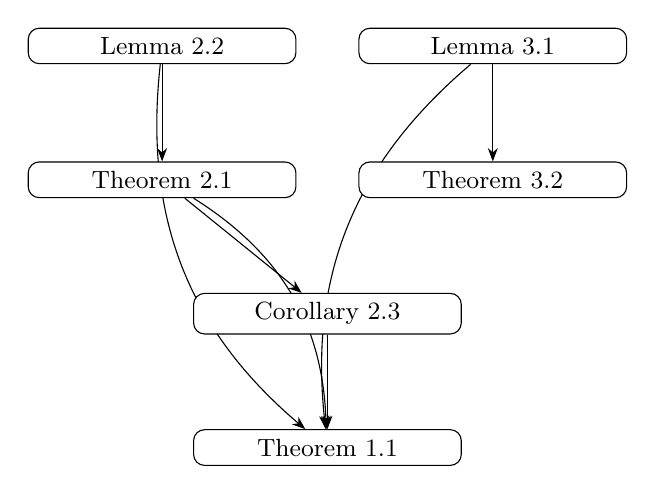
\begin{tikzpicture}[box/.style={draw,rounded corners,align=center,minimum width=34mm,font=\small,fill=white}, >=Stealth]
\node[box] (LEMMA001) at (-2.1,0.0) {Lemma 2.2};
\node[box] (LEMMA003) at (2.1,0.0) {Lemma 3.1};
\node[box] (LEMMA002) at (-2.1,-1.7) {Theorem 2.1};
\node[box] (LEMMA005) at (2.1,-1.7) {Theorem 3.2};
\node[box] (LEMMA004) at (0.0,-3.4) {Corollary 2.3};
\node[box] (CLAIM001) at (0.0,-5.1) {Theorem 1.1};
\begin{scope}[on background layer]
\draw[->, bend right=28] (LEMMA001) to (CLAIM001);
\draw[->, bend left=28] (LEMMA002) to (CLAIM001);
\draw[->, bend right=28] (LEMMA003) to (CLAIM001);
\draw[->] (LEMMA004) to (CLAIM001);
\draw[->] (LEMMA001) to (LEMMA002);
\draw[->] (LEMMA002) to (LEMMA004);
\draw[->] (LEMMA003) to (LEMMA005);
\end{scope}
\end{tikzpicture}
\end{center}
\section{Formalization}
Lean identifiers below are cross-references; the mathematics is in the sections above (\S{}29).
\subsection*{results\_eliahou\_theorem\_1\_1}
{\footnotesize\ttfamily\raggedright\hangindent=1.4em\hangafter=1\noindent
\hspace*{0.00em}theorem results\_\allowbreak{}eliahou\_\allowbreak{}theorem\_\allowbreak{}1\_\allowbreak{}1 \{L : \ensuremath{\mathbb{N}}\} (c : CollatzCycle L)\par
\hspace*{2.20em}(hinj : Function.\allowbreak{}Injective c.\allowbreak{}seq)\par
\hspace*{2.20em}(hmin : (2 : \ensuremath{\mathbb{N}}) \textasciicircum{} 40 < c.\allowbreak{}minElem) :\par
\hspace*{2.20em}\ensuremath{\exists} (a b cCoeff : \ensuremath{\mathbb{N}}), 0 < b \ensuremath{\wedge} a * cCoeff = 0 \ensuremath{\wedge}\par
\hspace*{3.30em}(Finset.\allowbreak{}univ.\allowbreak{}image c.\allowbreak{}seq).\allowbreak{}card =\par
\hspace*{4.40em}301994 * a + 17087915 * b + 85137581 * cCoeff\par
}

\section{Semantic Bridge}
\subsection*{Informal Statement}
Let \ensuremath{\Omega} be a nontrivial cycle of T. Provided min \ensuremath{\Omega} > 2\textasciicircum{}40, we have Card \ensuremath{\Omega} = 301994a + 17087915b + 85137581c, where a,b,c are nonnegative integers, b>0, and ac=0. In particular, the smallest admissible values for Card \ensuremath{\Omega} are 17087915, 17389909, 17691903, and so on.
\subsection*{Normalized Statement}
\subsection*{Normalized Claim: CLAIM-001 (Eliahou's Theorem 1.1)}
This statement must be understandable without reading any Lean code.

\subsubsection*{Objects and domains}
\begin{itemize}
\item $T : \mathbb{N} \to \mathbb{N}$, $T(n) = \begin{cases} n/2 & n \text{ even} \\ (3n+1)/2 & n \text{ odd} \end{cases}$ --- the ``compressed'' Collatz map (odd step and the forced halving folded into one step).
\item For $n \in \mathbb{N}$, the \textbf{trajectory} $\Omega(n) = \{n, T(n), T^{(2)}(n), \dots\} \subseteq \mathbb{N}$ (a \emph{set}, not a sequence).
\item $\Omega$ is a \textbf{cycle of length $k$} if $T^{(k)}(x) = x$ for every $x \in \Omega$, where \textbf{$k$ is defined to equal $\mathrm{Card}\,\Omega$} --- this is a definitional identity in the source, not a separately-proved fact.
\item $\Omega_1 := \{x \in \Omega : x \text{ odd}\}$.
\item The \textbf{trivial cycle} is $\Omega(1) = \{1, 2\}$; a cycle is \textbf{nontrivial} iff it is not this set.
\item $\theta := \log_2(3) \in \mathbb{R}$, irrational (elementary: $3$ is not a power of $2$).
\item $(p_n/q_n)_{n \ge 0}$: the principal convergents to $\theta$ from its continued-fraction expansion, via the standard recursion $p_n = a_n p_{n-1} + p_{n-2}$, $q_n = a_n q_{n-1} + q_{n-2}$.
\item Two fractions $(p/q), (p'/q')$ (nonnegative integers) form a \textbf{Farey pair} if $pq' - p'q = \pm 1$.
\end{itemize}
\subsubsection*{The claim}
\textbf{Given}: $\Omega$ a nontrivial cycle of $T$, with $\min \Omega > 2^{40}$.

\textbf{Conclusion}: there exist nonnegative integers $a, b, c$ with $b > 0$ and $ac = 0$ such that

\[ \mathrm{Card}\,\Omega = 301994\,a + 17087915\,b + 85137581\,c. \]
The three constants are not arbitrary --- they are specific convergents of $\theta = \log_2 3$: $p_{13} = 301994$, $p_{15} = 17087915$, $p_{16} = 85137581$.

\subsubsection*{Why this is true (the actual argument, normalized)}
1. From an earlier result (the ``sandwich inequality'', $\mathrm{Card}\,\Omega / \mathrm{Card}\,\Omega_1 \in (\log_2(3+1/M), \log_2(3+1/m)]$ where $m=\min\Omega, M=\max\Omega$), and the hypothesis $\min\Omega > 2^{40}$, one gets $k/l \in [\log_2 3,\ \log_2(3+2^{-40})]$ where $k=\mathrm{Card}\,\Omega,\ l=\mathrm{Card}\,\Omega_1$.

2. Numerically (via the continued-fraction machinery), that whole interval is sandwiched strictly between three specific convergents: $p_{16}/q_{16} < \log_2 3 < p_{15}/q_{15} < \log_2(3+2^{-40}) < p_{13}/q_{13}$.

3. So $k/l$ must land in one of exactly three places relative to those convergents, and a general lemma about Farey pairs (any fraction strictly between two Farey-paired fractions $p/q, p'/q'$ has the form $(ap+bp')/(aq+bq')$ for positive integers $a,b$) forces $k$ into one of three linear forms:

\begin{itemize}
\item between $p_{16}/q_{16}$ and $p_{15}/q_{15}$: $k = 17087915\,b + 85137581\,c$
\item exactly $p_{15}/q_{15}$: $k = 17087915\,b$
\item between $p_{15}/q_{15}$ and $p_{13}/q_{13}$: $k = 301994\,a + 17087915\,b$
\end{itemize}
4. Every case includes a nonzero $b$-term (hence $b>0$ always), and no case ever produces both a nonzero $a$ and a nonzero $c$ (hence $ac=0$). Combining the three cases into one statement gives exactly the claimed form.

\subsubsection*{Important disambiguation (not obvious from the statement alone)}
\begin{itemize}
\item "$\mathrm{Card}\,\Omega$" is genuinely a \textbf{set cardinality} --- $\Omega$ is a set of distinct positive integers, and the cycle ``length'' $k$ is \emph{defined} to be that cardinality, not an independently-chosen index count that merely happens to match it. Any formalization that represents a cycle via an indexed sequence of length $L$ must separately establish that the sequence is injective before $L$ can be identified with $\mathrm{Card}\,\Omega$ --- this is not free.
\item Yoneda's computational verification of the Collatz conjecture up to $2^{40}$ (cited only in the paper's introduction) is \textbf{not} a hypothesis of this theorem's proof. It explains why "$\min\Omega > 2^{40}$" is the interesting remaining case, but the proof of Theorem 1.1 does not depend on that computation being correct.
\end{itemize}
\subsubsection*{Status}
\textbf{MATCH} --- this normalization is a direct, complete restatement of the source's Theorem 1.1 and its proof (Sections 2-4 of the paper), independently re-derived from the primary source text (all 12 pages read), not copied from any secondary description (Lean repo README, prior AI summary, etc.). No part of the source's argument was found incoherent, circular, or underspecified.


\subsection*{Lean Statement}
{\footnotesize\ttfamily\raggedright\hangindent=1.4em\hangafter=1\noindent
\hspace*{0.00em}theorem results\_\allowbreak{}eliahou\_\allowbreak{}theorem\_\allowbreak{}1\_\allowbreak{}1 \{L : \ensuremath{\mathbb{N}}\} (c : CollatzCycle L)\par
\hspace*{2.20em}(hinj : Function.\allowbreak{}Injective c.\allowbreak{}seq)\par
\hspace*{2.20em}(hmin : (2 : \ensuremath{\mathbb{N}}) \textasciicircum{} 40 < c.\allowbreak{}minElem) :\par
\hspace*{2.20em}\ensuremath{\exists} (a b cCoeff : \ensuremath{\mathbb{N}}), 0 < b \ensuremath{\wedge} a * cCoeff = 0 \ensuremath{\wedge}\par
\hspace*{3.30em}(Finset.\allowbreak{}univ.\allowbreak{}image c.\allowbreak{}seq).\allowbreak{}card =\par
\hspace*{4.40em}301994 * a + 17087915 * b + 85137581 * cCoeff\par
}

\subsection*{Differences}
\subsection*{Gate 4: Lean Formalization Comparison}
Comparing \texttt{NORMALIZED-001} (independently derived from the source PDF) against

\texttt{Collatz/LinearForm.lean}'s \texttt{eliahou\_theorem\_1\_1} (and \texttt{Results.lean}'s

\texttt{results\_eliahou\_theorem\_1\_1} wrapper), in the target repo

\texttt{tangentstorm/eliahou-collatz-bounds} @ \texttt{db804ce6}.

\subsubsection*{Side-by-side}
\begin{center}\small\begin{tabular}{p{0.46\textwidth}p{0.46\textwidth}}\toprule
Human mathematics (normalized) & Lean \\ \midrule
$\Omega$ nontrivial cycle, $\min\Omega > 2^{40}$ & \texttt{(cyc : CollatzCycle L) (hinj : Function.Injective cyc.seq) (hmin : 2\textasciicircum{}40 < cyc.minElem)} \\
$\mathrm{Card}\,\Omega$ & \texttt{(Finset.univ.image cyc.seq).card} \\
$\exists\, a,b,c\ge 0,\ b>0,\ ac=0:\ \mathrm{Card}\,\Omega = 301994a+17087915b+85137581c$ & \texttt{\ensuremath{\exists} a b cCoeff : \ensuremath{\mathbb{N}}, 0 < b \ensuremath{\wedge} a * cCoeff = 0 \ensuremath{\wedge} (Finset.univ.image cyc.seq).card = 301994*a + 17087915*b + 85137581*cCoeff} \\
\bottomrule\end{tabular}\end{center}
\subsubsection*{Proof-structure comparison (not just the final statement)}
\begin{center}\small\begin{tabular}{p{0.46\textwidth}p{0.46\textwidth}}\toprule
Paper (p.55-56) & Lean (\texttt{Collatz/LinearForm.lean}) \\ \midrule
Lemma 3.1 (Farey intermediate fraction) & \texttt{farey\_intermediate\_coeffs} --- same hypotheses (Farey pair, strict betweenness), same conclusion form \\
$p_{16}/q_{16} < \log_2 3 < p_{15}/q_{15} < \log_2(3+2^{-40}) < p_{13}/q_{13}$ & \texttt{conv16\_lt\_logb\_three}, \texttt{farey\_15\_16}, \texttt{farey\_13\_15}, \texttt{logb\_three\_plus\_lt\_conv13} --- same chain of inequalities, same specific convergents \\
Three-way case split on where $k/l$ falls & \texttt{rcases lt\_trichotomy ((L:\ensuremath{\mathbb{Q}})/k\ensuremath{_{1}}) (17087915/10781274)} --- same trichotomy, same pivot fraction ($p_{15}/q_{15}$) \\
Case (i): $k/l\in(p_{16}/q_{16},p_{15}/q_{15}) \Rightarrow k=p_{15}b+p_{16}c$ & \texttt{hlt} branch: \texttt{farey\_intermediate\_coeffs} with \texttt{farey\_15\_16}, returns \texttt{\ensuremath{\langle}0, bCoeff, cCoeff, ...\ensuremath{\rangle}} \\
Case (ii): $k/l=p_{15}/q_{15} \Rightarrow k=p_{15}b$ & \texttt{heq} branch: divisibility argument via coprimality, returns \texttt{\ensuremath{\langle}0, b, 0, ...\ensuremath{\rangle}} \\
Case (iii): $k/l\in(p_{15}/q_{15},p_{13}/q_{13}) \Rightarrow k=p_{13}a+p_{15}b$ & \texttt{hgt} branch: \texttt{farey\_intermediate\_coeffs} with \texttt{farey\_13\_15}, returns \texttt{\ensuremath{\langle}bF, aF, 0, ...\ensuremath{\rangle}} \\
\bottomrule\end{tabular}\end{center}
\textbf{The Lean proof is not merely a different route to the same numbers --- it implements the same three-case Farey-pair argument, pivoting on the same convergent, using the same Farey identity, in the same order.}

\subsubsection*{Detected semantic differences (per Gate 4's required checklist)}
\begin{center}\small\begin{tabular}{p{0.46\textwidth}p{0.46\textwidth}}\toprule
Check & Finding \\ \midrule
Stronger/weaker statement & Neither --- see injectivity note below \\
Altered domain & No \\
Missing hypothesis & No --- \texttt{hinj} is \emph{additional}, not missing; see below \\
Extra hypothesis & \texttt{hinj : Function.Injective cyc.seq} --- see justification \\
Changed quantifier & No \\
Changed equality & No \\
Changed function & No \\
Changed coercion & \texttt{\ensuremath{\mathbb{R}}}/\texttt{\ensuremath{\mathbb{Q}}} intermediate steps (\texttt{rat\_of\_real\_div\_lt}) not present in the paper's argument, which works in $\mathbb{R}$ throughout --- a formalization convenience (rational arithmetic is decidable/computable where real arithmetic isn't), not a semantic change: the paper's own convergents are already rational by construction \\
Finite/infinite mismatch & No \\
Exact/approximate mismatch & No \\
\bottomrule\end{tabular}\end{center}
\subsubsection*{The one real structural difference: injectivity}
The paper's own definition (p.45) makes "cycle of length $k$" mean $k=\mathrm{Card}\,\Omega$ \textbf{by definition} --- a paper ``cycle'' is inherently what Lean calls an \texttt{ExactCollatzCycle} (injective indexing). Lean's base \texttt{CollatzCycle L} structure is strictly more general (it permits repeated elements within one period), so \texttt{eliahou\_theorem\_1\_1} adds \texttt{hinj} as an explicit hypothesis to recover exactly the paper's object of study.

This is \textbf{not} a weakening (the theorem isn't proved for a smaller class of paper-cycles) and \textbf{not} a strengthening (it isn't proved for objects the paper didn't consider) --- the injectivity hypothesis exactly closes the gap between Lean's more general indexed structure and the paper's implicit assumption. Confirmed independently in this session's prior audit (\texttt{evidence/semantic-audit-eliahou.md}) via the proved bridge lemma \texttt{ExactCollatzCycle.card\_eq\_length}.

\subsubsection*{Semantic status}
\textbf{MATCH.}


Syntactic signals in the Lean statement that a reviewer must address: injectivity ['Function.Injective'], finite\_structure ['.card', 'Finset'], strictness ['<'].
\subsection*{Findings recorded by the reviewer}
\begin{itemize}
\item \textbf{added hypotheses} (disclosed): hinj : Function.Injective cyc.seq is an extra hypothesis of the Lean theorem that the paper does not state (Gate 4: 'Extra hypothesis'); it is the encoding hypothesis, see Section 31 disclosure.
\item \textbf{coercions} (disclosed): The proof passes through R/Q intermediate steps (rat\_of\_real\_div\_lt) that the paper does not need; this is in the proof, not in the headline statement, and Gate 4 records it as a formalization convenience because the convergents are already rational.
\item \textbf{injectivity assumptions} (disclosed): hinj : Function.Injective cyc.seq. The paper defines cycle length k as Card Omega (p.45); Lean's CollatzCycle L is an L-indexed sequence that may repeat elements, so injectivity is required to identify L with Card Omega.
\item \textbf{classical assumptions} (disclosed): Classical.choice is in the axiom footprint (Gate 6). The Gate 7 note attributes it to ordinary real-number order decidability (Real.logb, lt\_trichotomy), as in any Mathlib real-analysis argument.
\end{itemize}
\subsection*{Justification}
Gate 4 records MATCH with one structural difference, injectivity: the injectivity hypothesis exactly closes the gap between Lean's more general indexed structure and the paper's definition, so the theorem is neither weakened nor strengthened relative to the paper. The proof also implements the paper's own three-case Farey-pair argument. The remaining disclosed items are the R/Q intermediate steps in the proof and Classical.choice in the footprint.


\subsection*{Representational difference (Section 31)}
\begin{description}
\item[What the object means informally.] Omega is a set of distinct positive integers forming a cycle of the compressed Collatz map T, and the paper defines the cycle's length k to equal Card Omega (p.45).
\item[What Lean's type represents.] cyc : CollatzCycle L, an L-indexed sequence cyc.seq (period L, repetitions allowed); Omega is the Finset (Finset.univ.image cyc.seq) and Card Omega is its .card.
\item[Why the encoding is valid.] With hinj : Function.Injective cyc.seq the indexing is exactly Lean's ExactCollatzCycle (injective indexing), which is what a paper 'cycle' inherently is; Gate 4 notes this was confirmed independently.
\item[Where the property is preserved.] Card Omega is the .card of the image finset in the conclusion; injectivity is what makes that image's size equal the period L.
\item[Whether the equality is literal or transported through an equivalence.] Literal on the image finset: the conclusion states an equality of natural numbers about (Finset.univ.image cyc.seq).card. The step from the paper's set Omega to the indexed sequence is the representational choice, not a transport through an equivalence.
\item[Assumptions that make the translation valid.] hinj (injective indexing) as an explicit theorem hypothesis, and hmin : 2\textasciicircum{}40 < cyc.minElem for the paper's minimum condition.
\end{description}
\subsection*{Verdict}
\noindent\textbf{FAITHFUL WITH EXPLICIT REPRESENTATIONAL DIFFERENCE}\par Set by Wilson. Recorded context: Gate 4 recorded MATCH; Gate 7 recorded PASS -- no undisclosed semantic change; Lean proves numOdd\_pos rather than assuming it (stricter than paper).
\section{Lean Environment}
\begin{tabular}{@{}ll@{}}
\toprule
Lean Version & 4.28.0 \\
Mathlib Version & v4.28.0 pin \\
\bottomrule
\end{tabular}
\section{Formal Verification}
PASS (8033/8033 jobs; see prior receipt for full log).
Source of this field: ledger:EVENT-006.
\section{Axiom Audit}
Actual axiom footprint: Classical.choice, Quot.sound, propext  [reported: Classical.choice].
Source: record:axiom-audit-record.json.
Classical.choice is present: the proof is classical, which is reported here and does not by itself fail the audit (\S{}14).
\section{Independent Check}
INDEPENDENTLY\_CHECKED -- 17464 declarations re-checked, axioms match Gate 6.
Recording the checker and its version does not by itself establish independence (\S{}17).
\section{Computational / Adversarial Tests}
Counterexample search: COMPUTATIONALLY\_SUPPORTED -- all convergents (p13,p15,p16), both Farey identities, and all three boundary inequalities confirmed. Original MISMATCH was a float64 precision artifact in the test script, not a defect in the claim. [diagnostic, not proof]

Computational test: COMPUTATIONALLY\_SUPPORTED -- see EVENT-010 [diagnostic, not proof]

Neither result is formal proof (\S{}16, \S{}18).
\subsection*{What these tests do not establish}
\begin{itemize}
\item They are not proof of the claim (Sections 16 and 18). A search that finds no counterexample is diagnostic evidence only.
\item The tested domain is not recorded for these results, so this report cannot say which cases were examined.
\item No counterexample was sought against the underlying claim about nontrivial Collatz cycles: doing so would require exhibiting an actual nontrivial cycle, which is computationally infeasible and open-problem-adjacent. The computational checks covered numeric and boundary structure only: the convergents p13, p15 and p16, both Farey identities, and the three boundary inequalities. (stated by Wilson)
\end{itemize}
\section{Verification Limitations}
\begin{longtable}{p{0.16\textwidth}p{0.78\textwidth}}
\toprule Item & Limitation \\ \midrule \endhead
1 & The proof uses Classical.choice; it is a classical proof. \\
2 & The repository, commit and toolchain were captured after the run (on 2026-09-19), not recorded during it; they describe the project as it is now, and the commit matches the one named in the run's own notes. \\
3 & The recorded result of EVENT-006 refers to a log or receipt that is not part of this report (``see prior receipt for full log''), so that material cannot be inspected here. \\
4 & No counterexample was sought against the underlying claim about nontrivial Collatz cycles: doing so would require exhibiting an actual nontrivial cycle, which is computationally infeasible and open-problem-adjacent. The computational checks covered numeric and boundary structure only: the convergents p13, p15 and p16, both Farey identities, and the three boundary inequalities (stated by Wilson). \\
5 & The independent check (Gate 9) ran patched copies of both external tools: lean4export and nanoda with a faster decimal conversion/parse of large number literals, because this proof contains literals of up to 25.6 million digits. The patches touch text conversion only, not type-checking, and were tested (identical export prefix, five earlier passes reproduce, a corrupted literal is rejected). The patched builds exist only on the recording machine; the two diffs are published beside the run (stated by Wilson). \\
\midrule \multicolumn{2}{l}{\textit{Record-keeping notes (these do not change what the verification shows)}} \\ \midrule
6 & 12 of 17 ledger events predate the input/output hash fields and carry none. \\
7 & Events EVENT-009 (MISMATCH\_FOUND); EVENT-010, EVENT-012 (COMPUTATIONALLY\_SUPPORTED) used wording outside the Section 16 vocabulary; each is read as diagnostic evidence, not proof. \\
\bottomrule
\end{longtable}
\section{Verification Matrix}
\begin{longtable}{lllll}
\toprule Gate & Ledger action & Event & Status & Satisfied \\ \midrule \endhead
G0 & source intake & EVENT-001 & PASS & yes \\
G1 & claim extraction & EVENT-013 & PASS & yes \\
G2 & assumption extraction & EVENT-003 & PASS & yes \\
G3 & semantic normalization & EVENT-004 & PASS & yes \\
G4 & lean formalization comparison & EVENT-005 & PASS & yes \\
G5 & lean build & EVENT-006 & PASS & yes \\
G6 & axiom audit & EVENT-007 & PASS & yes \\
G7 & semantic re audit & EVENT-008 & PASS & yes \\
G8 & adversarial computational test & EVENT-010 & DIAGNOSTIC & yes \\
G9 & independent check & EVENT-014 & PASS & yes \\
G10 & computational check & EVENT-012 & DIAGNOSTIC & yes \\
G11 & evidence graph & EVENT-015 & PASS & yes \\
G12 & report generation & EVENT-017 & PASS & yes \\
ORDER & canonical chain (\S{}2) & - & PASS & yes \\
\bottomrule
\end{longtable}
\section{Trust / Verification Chain}
\begin{center}
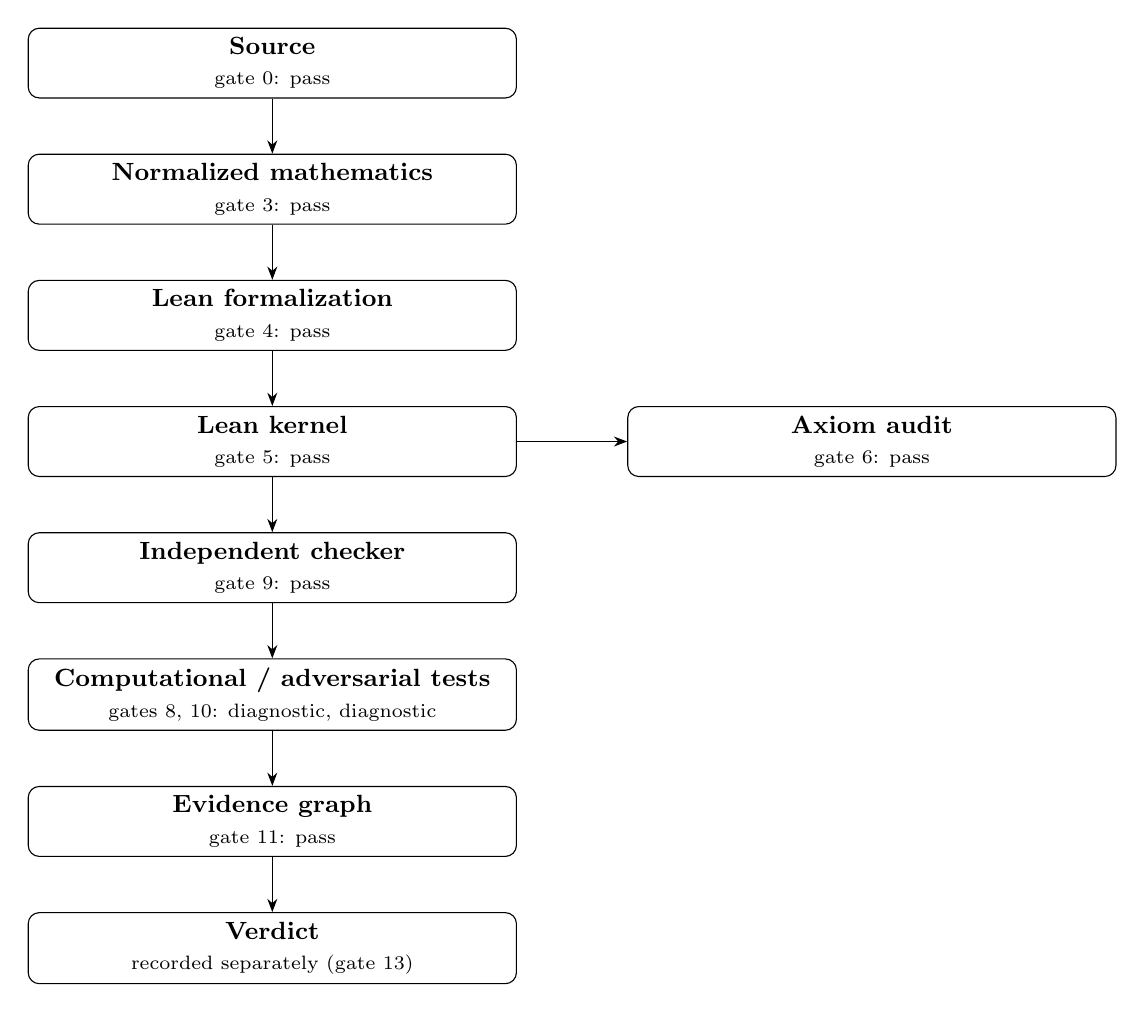
\begin{tikzpicture}[node distance=7mm, box/.style={draw,rounded corners,align=center,minimum width=62mm,font=\small}, >=Stealth]
\node[box] (src) {\textbf{Source}\\{\scriptsize gate 0: pass}};
\node[box, below=of src] (norm) {\textbf{Normalized mathematics}\\{\scriptsize gate 3: pass}};
\draw[->] (src) -- (norm);
\node[box, below=of norm] (lean) {\textbf{Lean formalization}\\{\scriptsize gate 4: pass}};
\draw[->] (norm) -- (lean);
\node[box, below=of lean] (kern) {\textbf{Lean kernel}\\{\scriptsize gate 5: pass}};
\draw[->] (lean) -- (kern);
\node[box, below=of kern] (chk) {\textbf{Independent checker}\\{\scriptsize gate 9: pass}};
\draw[->] (kern) -- (chk);
\node[box, below=of chk] (comp) {\textbf{Computational / adversarial tests}\\{\scriptsize gates 8, 10: diagnostic, diagnostic}};
\draw[->] (chk) -- (comp);
\node[box, below=of comp] (evd) {\textbf{Evidence graph}\\{\scriptsize gate 11: pass}};
\draw[->] (comp) -- (evd);
\node[box, below=of evd] (ver) {\textbf{Verdict}\\{\scriptsize recorded separately (gate 13)}};
\draw[->] (evd) -- (ver);
\node[box, right=14mm of kern] (ax) {\textbf{Axiom audit}\\{\scriptsize gate 6: pass}};
\draw[->] (kern) -- (ax);
\end{tikzpicture}
\end{center}
\section{Reproducibility Instructions}
\begin{tabular}{@{}p{0.27\textwidth}p{0.68\textwidth}@{}}
\toprule
Repository URL & https://github\allowbreak{}.com/tangentst\allowbreak{}orm/eliahou-co\allowbreak{}llatz-bounds.g\allowbreak{}it \\
Commit & db804ce6305ea9\allowbreak{}9a817f06786960\allowbreak{}7f8b677d895a (working tree clean) \\
Project directory (now) & /Users/lordwil\allowbreak{}son/ico-collat\allowbreak{}z/targets/elia\allowbreak{}hou-collatz-bo\allowbreak{}unds \\
Lean toolchain file & leanprover/lea\allowbreak{}n4:v4.28.0 \\
Lean version & 4.28.0 \\
Lake version & Lake version 5.0.0-src+7e01\allowbreak{}a1b (Lean version 4.28.0) \\
Mathlib revision & v4.28.0 pin (commit 8f9d9cff6bd728\allowbreak{}b17a24e163c940\allowbreak{}2775d9e6a365) \\
Checker & nanoda 4c544ed4099c82\allowbreak{}27f07d5de77ad1\allowbreak{}e69fb0740a27, export format 3.1.0 \\
Expected build result & PASS (8033/8033 jobs; see prior receipt for full log) \\
How these were obtained & Captured 2026-09-19 from the project as it is now; not recorded during the run \\
Matches the commit the run's notes name & yes (db804ce6) \\
\bottomrule
\end{tabular}

{\footnotesize\ttfamily\raggedright\hangindent=1.4em\hangafter=1\noindent
\hspace*{0.00em}git clone https:/\allowbreak{}/\allowbreak{}github.\allowbreak{}com/\allowbreak{}tangentstorm/\allowbreak{}eliahou-collatz-bounds.\allowbreak{}git\par
\hspace*{0.00em}cd eliahou-collatz-bounds\par
\hspace*{0.00em}git checkout db804ce6305ea99a817f067869607f8b677d895a\par
\hspace*{0.00em}cat lean-toolchain\par
\hspace*{0.00em}lake --version\par
\hspace*{0.00em}lean --version\par
\hspace*{0.00em}lake exe cache get \&\& lake build\par
\hspace*{0.00em}\# in a Lean file importing the module:  \#print axioms results\_\allowbreak{}eliahou\_\allowbreak{}theorem\_\allowbreak{}1\_\allowbreak{}1\par
\hspace*{0.00em}\# independent check (paths are those of the recording machine):\par
\hspace*{0.00em}cd /\allowbreak{}Users/\allowbreak{}lordwilson/\allowbreak{}ico-collatz/\allowbreak{}targets/\allowbreak{}eliahou-collatz-bounds \&\& lake env /\allowbreak{}Users/\allowbreak{}lordwilson/\allowbreak{}ico-collatz/\allowbreak{}targets/\allowbreak{}lean4export-fastnat/\allowbreak{}.\allowbreak{}lake/\allowbreak{}build/\allowbreak{}bin/\allowbreak{}lean4export Results -- results\_\allowbreak{}eliahou\_\allowbreak{}theorem\_\allowbreak{}1\_\allowbreak{}1 > results\_\allowbreak{}eliahou\_\allowbreak{}theorem\_\allowbreak{}1\_\allowbreak{}1.\allowbreak{}export\par
\hspace*{0.00em}/\allowbreak{}Users/\allowbreak{}lordwilson/\allowbreak{}ico-collatz/\allowbreak{}targets/\allowbreak{}nanoda\_\allowbreak{}lib-fastparse/\allowbreak{}target/\allowbreak{}release/\allowbreak{}nanoda\_\allowbreak{}bin results\_\allowbreak{}eliahou\_\allowbreak{}theorem\_\allowbreak{}1\_\allowbreak{}1.\allowbreak{}nanoda-config.\allowbreak{}json\par
}

The repository facts were captured after the run and describe the project as it is now; they do not prove what the original run built. The build command is the one recorded in EVENT-006.
Reproducibility level supported by recorded evidence: R4. This tool did not re-run the build.
\section{Correction Ledger}
\begin{itemize}
\item \textbf{TEST-001} (EVENT-009): MISMATCH\_FOUND (p16/q16 < log2(3) boundary check failed under float64 precision)
\end{itemize}
\subsection*{Correction Ledger --- VCE-001 rev s}
\subsubsection*{CORRECTION-001 --- claims extraction EVENT-002 superseded by EVENT-013}
\begin{itemize}
\item \textbf{original\_claim}: the delivered VCE-001 \texttt{claims.json} (EVENT-002) stated the extraction of Theorem 1.1 accurately.
\item \textbf{error}: a ``fact the statement relies on'' mixed up K(2\textasciicircum{}39) = p\_13 with K(2\textasciicircum{}40) = p\_15 in one sentence, and proof step 2 called the interval for k/l ``closed-open-ish'' when Theorem 2.1 gives the open interval (log2(3), log2(3+2\textasciicircum{}-40)).
\item \textbf{detection\_method}: reading the extraction against the source (p.55, Theorem 2.1).
\item \textbf{root\_cause}: hand-written working notes kept in the extraction.
\item \textbf{repair}: Wilson confirmed two edits (2026-09-19); the cleaned file is \texttt{claims-v2/claims.json}; EVENT-013 supersedes EVENT-002. The delivered \texttt{claims.json} is unchanged.
\item \textbf{recheck}: \texttt{validate-claims} passes; the rendered report was read.
\item \textbf{result}: RESOLVED. Nothing in the proof or conclusion changed.
\item \textbf{date}: 2026-09-19
\end{itemize}
\subsubsection*{CORRECTION-002 --- Gate 9 ``CHECKER\_INCOMPATIBLE'' (EVENT-011) superseded by EVENT-014; the recorded root cause was wrong}
\begin{itemize}
\item \textbf{original\_claim}: EVENT-011 recorded CHECKER\_INCOMPATIBLE for \texttt{results\_eliahou\_theorem\_1\_1} --- ``lean4export stalls on this theorem's large proof closure (reproducible, root-caused: memoization cache reset on every call in Export.lean, not a resource issue)''. Repeated in the delivered VCE-001 report and in the Phase 18 correction ledger and verifying-lean-proofs skill.
\item \textbf{error}: the stated root cause was a hypothesis (the Phase 18 ledger itself called it one) that had been repeated as established fact. It is not the cause. A stack sample of the stalled exporter shows the time in \texttt{Nat.reprFast} \ensuremath{\to} \texttt{toDigitsCore} \ensuremath{\to} \texttt{\_\_gmpn\_divrem\_1}: quadratic decimal conversion of a huge natural-number literal. The proof term contains literals of up to \textbf{25,628,966 digits} (81 literals above 50 digits). The stall was not a defect of the proof or a memoization bug, and the gap was fixable.
\item \textbf{detection\_method}: re-reading the archived \texttt{sample} output while starting the Gate 9 repair, instead of trusting the recorded cause.
\item \textbf{root\_cause}: (1) \texttt{lean4export} prints a natVal with \texttt{s!``\{i\}''}, i.e. \texttt{Nat.repr}, one digit at a time. (2) The checker, nanoda, parses the same literal with \texttt{BigUint::from\_str}, also quadratic, so fixing only the exporter moved the stall to the checker (observed: \texttt{from\_str\_radix} at 100\% CPU for 5+ minutes).
\item \textbf{repair}: two small patches, kept as diffs in \texttt{\textasciitilde{}/fcve/tool-patches/}: \texttt{lean4export-fast-natval.diff} (divide-and-conquer decimal conversion, same output as \texttt{Nat.repr}) and \texttt{nanoda-fast-decimal-parse.diff} (divide-and-conquer decimal parse, same value as \texttt{from\_str}). The unpatched tools are untouched; patched copies live in \texttt{targets/lean4export-fastnat} and \texttt{targets/nanoda\_lib-fastparse}. Patch diff sha256: exporter \texttt{11f0d0fc\ensuremath{\ldots}}, checker \texttt{5f946992\ensuremath{\ldots}}.
\item \textbf{recheck}: (a) the patched exporter's output is byte-identical to the original exporter's partial export over its first 71,147,000 bytes; (b) unit tests: exporter conversion vs \texttt{Nat.repr} on 3,000+ numbers and edge cases, 0 mismatches; checker parse vs \texttt{from\_str} on 45 random strings up to 300,000 digits incl. leading zeros, all equal; (c) \textbf{regression}: the patched checker re-checks the five theorems that passed with the original checker with identical declaration counts (12012, 12809, 13639, 17320, 17301); (d) \textbf{negative control}: changing one digit of one 25.6M-digit literal in the export makes the patched checker fail (panic on a failed \texttt{def\_eq}, exit 101); the untouched export passes; (e) the run itself: export complete (187,326,147 bytes, 60 s), nanoda ``Checked 17464 declarations with no errors'', checker axioms \{propext, Quot.sound, Classical.choice\} equal the Gate 6 footprint from a fresh machine-produced audit.
\item \textbf{result}: RESOLVED for Gate 9: INDEPENDENTLY\_CHECKED. \textbf{Disclosed limit:} the verdict comes from patched copies of both tools. The patches touch only decimal text conversion, not the type-checking logic, and were validated as above, but they are a change to the checker's trusted input path that a reviewer may wish to inspect (the diffs are 43 and 80 lines).
\item \textbf{date}: 2026-09-19
\item \textbf{side note}: the first attempt through \texttt{independent-check.sh} failed with ``failed to open configuration file'' because the script \texttt{cd}s before using a relative config path when \texttt{--out} is relative. That was a tooling error, not a verdict; the run was repeated through \texttt{fcve.py independent-check} with absolute paths.
\end{itemize}


\section{Conclusion}
The recorded evidence is summarized in the Trust Statement and the verification matrix above. Recorded failure is not a passed gate.
\begin{center}\begin{tabular}{@{}p{0.36\textwidth}p{0.58\textwidth}@{}}
FORMAL PROOF (build): & PASS \\
AXIOM AUDIT: & PASS \\
SEMANTIC MATCH (Gate 4): & PASS \\
SEMANTIC RE-AUDIT (Gate 7): & PASS \\
INDEPENDENT CHECK: & PASS \\
COUNTEREXAMPLE SEARCH: & NO COUNTEREXAMPLE FOUND IN TESTED DOMAIN (diagnostic, not proof) \\
COMPUTATIONAL TEST: & NO COUNTEREXAMPLE FOUND IN TESTED DOMAIN (diagnostic, not proof) \\
REPRODUCIBILITY: & R4 (ceiling supported by recorded evidence) \\
\end{tabular}\end{center}
%% PERMITTED-STATUS-BEGIN
\begin{quote}\textbf{Status the evidence permits.} The recorded evidence satisfies the conditions for promotion (Section 53). Whether to promote is the reviewer's decision, recorded after this report. This is not a decision: the governance decision is recorded as a separate step after this report.\end{quote}
%% PERMITTED-STATUS-END
\appendix
\section{Lean Source}
{\footnotesize\ttfamily\raggedright\hangindent=1.4em\hangafter=1\noindent
\hspace*{0.00em}theorem results\_\allowbreak{}eliahou\_\allowbreak{}theorem\_\allowbreak{}1\_\allowbreak{}1 \{L : \ensuremath{\mathbb{N}}\} (c : CollatzCycle L)\par
\hspace*{2.20em}(hinj : Function.\allowbreak{}Injective c.\allowbreak{}seq)\par
\hspace*{2.20em}(hmin : (2 : \ensuremath{\mathbb{N}}) \textasciicircum{} 40 < c.\allowbreak{}minElem) :\par
\hspace*{2.20em}\ensuremath{\exists} (a b cCoeff : \ensuremath{\mathbb{N}}), 0 < b \ensuremath{\wedge} a * cCoeff = 0 \ensuremath{\wedge}\par
\hspace*{3.30em}(Finset.\allowbreak{}univ.\allowbreak{}image c.\allowbreak{}seq).\allowbreak{}card =\par
\hspace*{4.40em}301994 * a + 17087915 * b + 85137581 * cCoeff\par
}

\section{Tests}
\begin{itemize}
\item \textbf{EVENT-009} python3 verification/computational/tests/verify\_convergents.py (initial run, native float boundary comparison): MISMATCH\_FOUND (p16/q16 < log2(3) boundary check failed under float64 precision)
\item \textbf{EVENT-010} python3 verification/computational/tests/verify\_convergents.py (corrected: mpf 60-digit precision for boundary comparisons): COMPUTATIONALLY\_SUPPORTED -- all convergents (p13,p15,p16), both Farey identities, and all three boundary inequalities confirmed. Original MISMATCH was a float64 precision artifact in the test script, not a defect in the claim.
\item \textbf{EVENT-012} Python/mpmath backend (per Section 19 backend abstraction; MATLAB not required): COMPUTATIONALLY\_SUPPORTED -- see EVENT-010
\end{itemize}
\section{Evidence Receipt}
\begin{longtable}{p{0.24\textwidth}p{0.70\textwidth}}
\toprule Field & Value \\ \midrule \endhead
SOURCE HASH & sha256:077292b\allowbreak{}ebdf53a6e06d92\allowbreak{}fb475ce395ee1c\allowbreak{}8af4cc3e9f5c2e\allowbreak{}4620b2e3513468\allowbreak{}9 (source/origin\allowbreak{}al.pdf) \\
THEOREM ID & CLAIM-001 (Theorem 1.1) \\
CLAIM & Let \ensuremath{\Omega} be a nontrivial cycle of T. Provided min \ensuremath{\Omega} > 2\textasciicircum{}40, we have Card \ensuremath{\Omega} = 301994a + 17087915b + 85137581c, where a,b,c are nonnegative integers, b>0, and ac=0. In particular, the smallest admissible values for Card \ensuremath{\Omega} are 17087915, 17389909, 17691903, and so on. \\
NORMALIZED CLAIM & normalized/nor\allowbreak{}malized-claim.\allowbreak{}md -- MATCH \\
LEAN STATEMENT & results\_eliaho\allowbreak{}u\_theorem\_1\_1 -- Gate 4: MATCH \\
LEAN VERSION & 4.28.0 \\
MATHLIB VERSION & v4.28.0 pin \\
BUILD RESULT & PASS (8033/8033 jobs; see prior receipt for full log) \\
AXIOM FOOTPRINT & Classical.choi\allowbreak{}ce, Quot.sound, propext  [reported: Classical.choi\allowbreak{}ce] \\
INDEPENDENT CHECK & INDEPENDENTLY\_\allowbreak{}CHECKED -- 17464 declarations re-checked, axioms match Gate 6 \\
COMPUTATIONAL TEST & COMPUTATIONALL\allowbreak{}Y\_SUPPORTED -- see EVENT-010 [diagnostic, not proof] \\
COUNTEREXAMPLE SEARCH & COMPUTATIONALL\allowbreak{}Y\_SUPPORTED -- all convergents (p13,p15,p16), both Farey identities, and all three boundary inequalities confirmed. Original MISMATCH was a float64 precision artifact in the test script, not a defect in the claim. [diagnostic, not proof] \\
SEMANTIC MATCH & Gate 4: MATCH; Gate 7: PASS -- no undisclosed semantic change; Lean proves numOdd\_pos rather than assuming it (stricter than paper) \\
REPRODUCIBILITY LEVEL & R4 (ceiling supported by recorded evidence; NOT re-run by this tool; R5 needs full-package rebuild, not assessed) \\
GRAPH HASH & v3 930efe7a5cf50d\allowbreak{}d3719bbf838882\allowbreak{}ca33bcde0ecbc1\allowbreak{}b6a6a4e13e4157\allowbreak{}3237708d (covers 17 events through EVENT-017) \\
COST & 17 ledger events; LEAN\_BUILD\_TIM\allowbreak{}E=NOT RECORDED; COMPUTATIONAL\_\allowbreak{}TEST\_TIME=NOT RECORDED; CHECKER\_TIME=6\allowbreak{}0.0; HUMAN\_TIME, MODEL\_CALL\_COU\allowbreak{}NT, MODEL\_COST, LATEX\_BUILD\_TI\allowbreak{}ME=NOT RECORDED (no cost ledger, \S{}43) \\
\bottomrule
\end{longtable}
\end{document}
